\documentclass[a4paper, 11pt]{article}
\usepackage[utf8]{inputenc}
\usepackage[T1]{fontenc}
\usepackage[french]{babel}
\usepackage[linkcolor=blue, colorlinks=true,]{hyperref}
\usepackage{graphicx}
\usepackage{fancyhdr}
\pagestyle{fancy}
\fancyhead[C]{\rightmark}
\fancyhead[L]{}
\fancyhead[R]{}
\fancyfoot[C]{\hyperlink {participation} {Envie de participer?}}

\makeatletter
\let\insertdate\@date
\makeatother

% Creare Mundum est sous licence CC-BY-SA, présente dans le dossier d'origine, merci de la respecter!

\title{Sombre, Sombre-Cime\\ Scénario pour Creare Mundum \\ Devel}
\author{The Creare Mundum Project}
\date{\oldstylenums{\insertdate}}
\begin{document}
\maketitle
\setcounter{tocdepth}{1} %Génération du Sommaire.
\renewcommand{\contentsname}{Sommaire} 
\tableofcontents
\newpage

%----------------------------------------------------------------------------
\section{Introduction pour le maitre de jeu}
"Sombre, Sombre-Cime" est un court scénario de trois à quatre heures. Il met en scène la mort des personnages, qu'un nécromancien utilise alors à ses fins. Ils seront sauvés par leur courage et l'aide d'un grand prêtre de l'ordre de la guérison, Monseigneur Torwar.
Cette intrigue prend place dans l'univers de Creare Mundum, durant l'ère médiévale. Pour plus de précisions concernant le monde, consultez le fichier principal.
\newline
Creare Mundum n'a pas de système de règle propre, il reste donc au maitre de jeu le travail d'adapter ce scénario au système qu'il souhaite utiliser, notamment e ce qui concerne la création des monstres.
\newline
Les paragraphes commençant par "Partie supplémentaire: " sont comme leur nom l'indique, hors de l'intrigue principale, mais permettent une plus grande immersion et un allongement du temps de jeu.
\newline
Les instructions et le déroulement qui suivent sont bien sûr donné uniquement à titre indicatif, n'hésitez pas à modifier cette aventure comme bon vous semble!

\section{Du vieil aulne au vieux chêne}
\subsection{Un départ}
L'action commence à la périphérie d'Anksfall. Les personnages se trouvent sur la place de l’aulne, lieu de départ de la plupart des voyages vers le nord. Nos héros ne se connaissent pas forcément, et leur arrivée un par un peut être un effet de style intéressant. C'est de cette place qu'une carriole doit vernir les prendre pour aller à Sombre-Cime. En effet, la "Grande Foire de Sombre-Cime" approche et les personnages y vont pour des motifs différents. Les personnages  se rencontrent donc sur cette petite place, qui n'as de place que le nom. Un grand aulne se dresse a coté de la grande route. Un petit abris a été dressé pour protéger les voyageurs. La scène du voyage est dédiée à la rencontre des personnages. Le voyage comporte peut de danger et dure une dizaine d'heure. Dans la carriole se trouve aussi trois chevaliers qui partent à la foire: Revir, Pegrus et Larsus. Étrangement, ils n'ont pas l'air festif, bien qu'ils démentiront quoi que ce soit si les héros leur posent des questions.

\subsection{Partie supplémentaire: L'attaque des gobelins} 
La compagnie est attaquée peu avant l'arrivée, sur une petite route qui coupe à travers un petit bois des plaines de sang, que le cocher assurait "sans danger". Un groupe composé d'autant de gobelins que de personnages plus 3 entre en combat. Ils ne sont pas particulièrement fort, ils manque des membres à certaines d'entre eux, et à leur mort, ils semblent comme retrouver le sourire. Il s'agit en fait de cobayes du nécromancien dont les héros seront les victimes. 

\subsection{Une arrivée}
Les héros arrivent en soirée ou au petit matin, la foire commence de toute façon le lendemain. Ils font ce qu'ils veulent, flâner dans les boutiques (la plupart on déjà leurs étalages de près), prendre une chambre d'hôtel, visiter la ville... S'ils approchent de l'église de la ville, dédiée à l'ordre du soin, ils y voient de l'agitation. Si les personnages cherchent à savoir pourquoi, en posant quelques questions, il apprendront vite qu'un des grands prêtres de l'ordre, Torwar, est ici pour célébrer une messe pour la foire. Faites durer cette partie autant que vous voulez, mais il faut faire attention à ne pas ennuyer les personnages.

\subsection{La mort est douce}
Cette partie est plus intéressante jouée dans une semi-obscurité. Les personnages vont y mourir, de la main d'un mystérieux spectre. Ils passent l'arme à gauche un par un, toutes les 5 minutes environ, quoiqu'ils fassent. Aidez-les dans leur fuite, conseillez-les, jouez sur leur ressentis: Suivez la voie qu'il tracent pour vous. Voici des exemples de ce qu'ils peuvent ressentir:
\begin{itemize}
\item "Tu sens une piqure dans le cou. Ton cœur ralentit, puis s’arrête"
\item  "Tu sens une piqure sur la jambe. Après avoir fait trois pas, elle se dérobe sous ton poids. Tu tombes, perdant connaissance. "
\item  "Une douleur atroce se propage dans ton corps, mais ta voix refuse de produire un son. Tu tombes par terre en gémissant. "
\end{itemize}

\section{Le château grotesque}
\subsection{Illusion}
Nos héros sont réveiller par des cris. Ils sont dans une chambre de princesse, sans doute en haut d'un donjon. La princesse, justement, leur cri de se préparer, qu' "Ils arrivent". En effet, des bruits se font entendre dans les escaliers. Les personnages ont justes le temps de se préparer, la porte explose, avec un nombre de hobgobelins égal à celui du nombre de joueur plus deux. Le combat éclate. Durant ce dernier, la princesse lance des sortilèges étrangement puissants, et les personnages se sentent comme immortels.

\subsection{Explication} 
Il faut savoir que les héros sont victimes d'un puissant sort d'illusion. La princesse est un nécromancien, les hobgobelins sont de nobles guerriers et les personnages des zombies du nécromancien (ce qui explique l'ascendant qu'il a sur leurs esprits). Ce dernier a donc créer une illusion pour que ses zombies l'aident à tuer les chevaliers. Si la princesse/nécromancien meurt, ou dès la fin du combat, d'étranges tâches sombres commencent à apparaitre sur les murs. L'illusion se rompt. Au bout de quelques tours, elle casse entièrement, les personnages se retrouvent alors dans une grotte.
\newline
Les chevaliers meurent ou gisent, mourants, aux pieds de nos héros. Ces derniers ne se rendent d’ailleurs pas immédiatement compte de leur état  cadavérique. Celui obtenant le meilleur score aux dés s'en rend compte: "Tiens, tu sens une très forte odeur de pourriture. Après quelques recherches olfactives, tu devines d'où elles viennent: de ton cadavre". Les personnages sont donc insensibles aux coups, mais supportent mal le soleil, et bien sûr, quiconque les voit fuit ou les attaque.
\newline
Quoiqu'il en soit, le nécromancien est soit mort, soit il attaque les personnages dès qu'il le peut après la fin du combat, ces derniers ne répondant plus à son pouvoir. Une fois définitivement mort, les personnages peuvent le fouiller pour en apprendre plus. Ils trouvent dans sa robe noire une \hyperlink{lettre}{lettre} (voir les ressources pour une meilleur qualité).

\begin{figure}[p]
\begin{center}
\hypertarget{lettre}{}
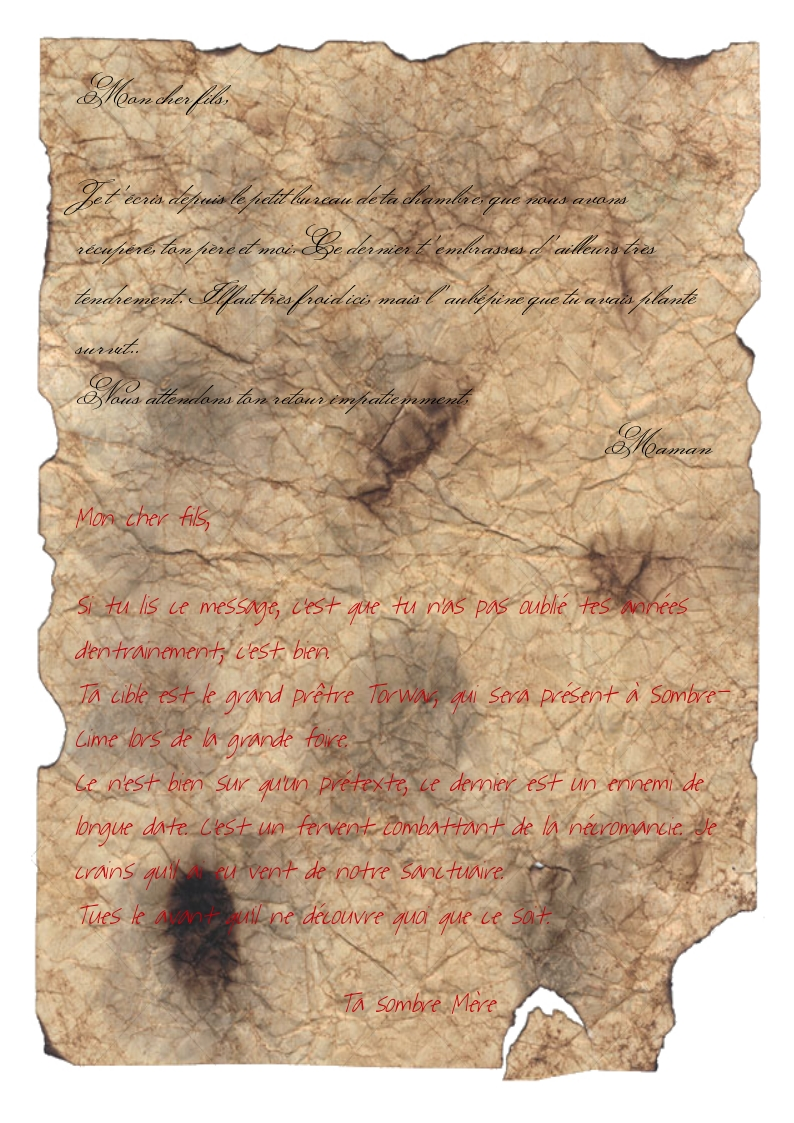
\includegraphics[scale=0.45]{./Ressources/lettre.jpg}
\caption{La lettre du nécromancien}
\end{center}
\end{figure}
S'ils cherchent un peu dans la grotte, ils trouveront une sorte de cercle composé de signes ésotériques, servant à la nécromancie. Les affaires du sorcier ne comprennent que quelques pièces d'or, ainsi que d'un plan détaillé de Sombre-Cime.

\section{La vie d'un cadavre est dure}
\subsection{Attention au départ}
Les personnages vont donc, selon toute vraisemblance, se rendre à l'église de Sombre-Cime pour aller voir le prêtre Torwar, seul capable de les aider.
Du fait de leur états de décomposition, les personnages vont devoir se protéger, se cacher durant le reste de l'histoire, sous peine de provoquer une émeute à leur encontre. L'idéal est de voyager de nuit.
\subsection{Partie supplémentaire: "Des... DES ZOMBIES"} 
Si les personnages oublient leur aspect repoussant, ou échouent à des tests de discrétions pour passer la porte de la ville par exemple, la garde de la ville est alertée, et les attaques s'ils ne quittent pas les lieux. Les personnages, insensible à la mort (sauf magique ou par décapitation) peuvent choisir de forcer le passage, ou de se replier. S'ils prennent la deuxième option, ils va falloir qu'ils reviennent une autre fois, en doublant d'adresse pour passer la garde, elle aussi doublée face à la menace.
\newline
Mais certains voleurs connaissent bien les souterrains de la ville, et, moyennant monnaie, peuvent faire passer nos héros dans la ville en toute discrétion.
\subsection{L'église de la guérison}
L'église Sombre-Cime est dédiée aux soins. Construite dans un style proche de l'art roman. De grandes colonnades soutiennent l'architecture. Il y a plusieurs petits autels qui entoure le maitre-autel. Chacun des ces petits autels sont dédiés à une forme particulière de la guérison : Celle de maladies, celle de blessures... Mais, une colonne à gauche est toute particulière. À ses extrémités se trouvent des encoches, juste assez larges pour laisser passer la colonne elle même. Dans le mur adjacent se trouve une petite ouverture, sans doute une serrure. Vous l'aurez compris, nous entrons ici dans une phase de recherche. Laissez les personnages déambuler, remarquer l'encoche et les rainures. Le but est donc de trouver une petite clé qui déplacera la colonne. Étrangement, personne ne semble remarquer que la colonne est déplaçable, ni même l'encoche dans le mur. De la puissante magie est derrière tout ça.

\subsection{Recherche}
Durant leur recherches, les personnages peuvent rencontrer :
\begin{itemize}
\item Le prêtre : "Le grand prêtre dort dans sa chambre, ne le dérangez pas mes fils". Le prêtre est vaguement au courant des activités du grand prêtre concernant la nécromancie. Si les personnages montrent leur état, le prêtre les conduits immédiatement dans la chambre du grand prêtre, mais ce dernier n'y ai pas. Le prêtre ne sais pas où il  a pu passer. Il n'as pu sortir, on l’aurait vu.
\item Dovos Jembar : "Oui, le grand prêtre Torwar est là pour bénir la foire de demain". Dovos est un retraité habitué de la paroisse.
\item Robith Brosas : "Le grand prêtre est là, où ça ? ". Robith est boulanger dans la ville et se soucie surtout de sa mère malade
\item Fantôme : S'il y a un sorcier ou un prêtre, ces derniers voient un ectoplasme qui se tiens prêt de la colonne de gauche. Dès que le fantôme remarque les personnages, il pointe la serrure dans le mur.
\end{itemize}

Il n'y a pas de solution à cette recherche. Au bout de la deuxième ou troisième bonne idée de la part de vos joueurs, la clé est trouvée.
\newline
Une fois que la clé a été tournée dans la serrure, la colonne se déplace en effet, dévoilant un étroit goulot d'une dizaine de mètre muni d'une échelle. Aucune des personnes étrangères au groupe d'investigateur ne remarquent quoique ce soit.

\section{Le temple dans le temple} 
\subsubsection{Les catacombes}
Après avoir descendu l'échelle (les autres personnes ne réagissent pas, la magie de dissimulation est vraiment très forte), les personnages se retrouvent dans un tunnel formé d'os en tout genre.

\begin{figure}[ht]
\begin{center}
\hypertarget{catacombes}{}
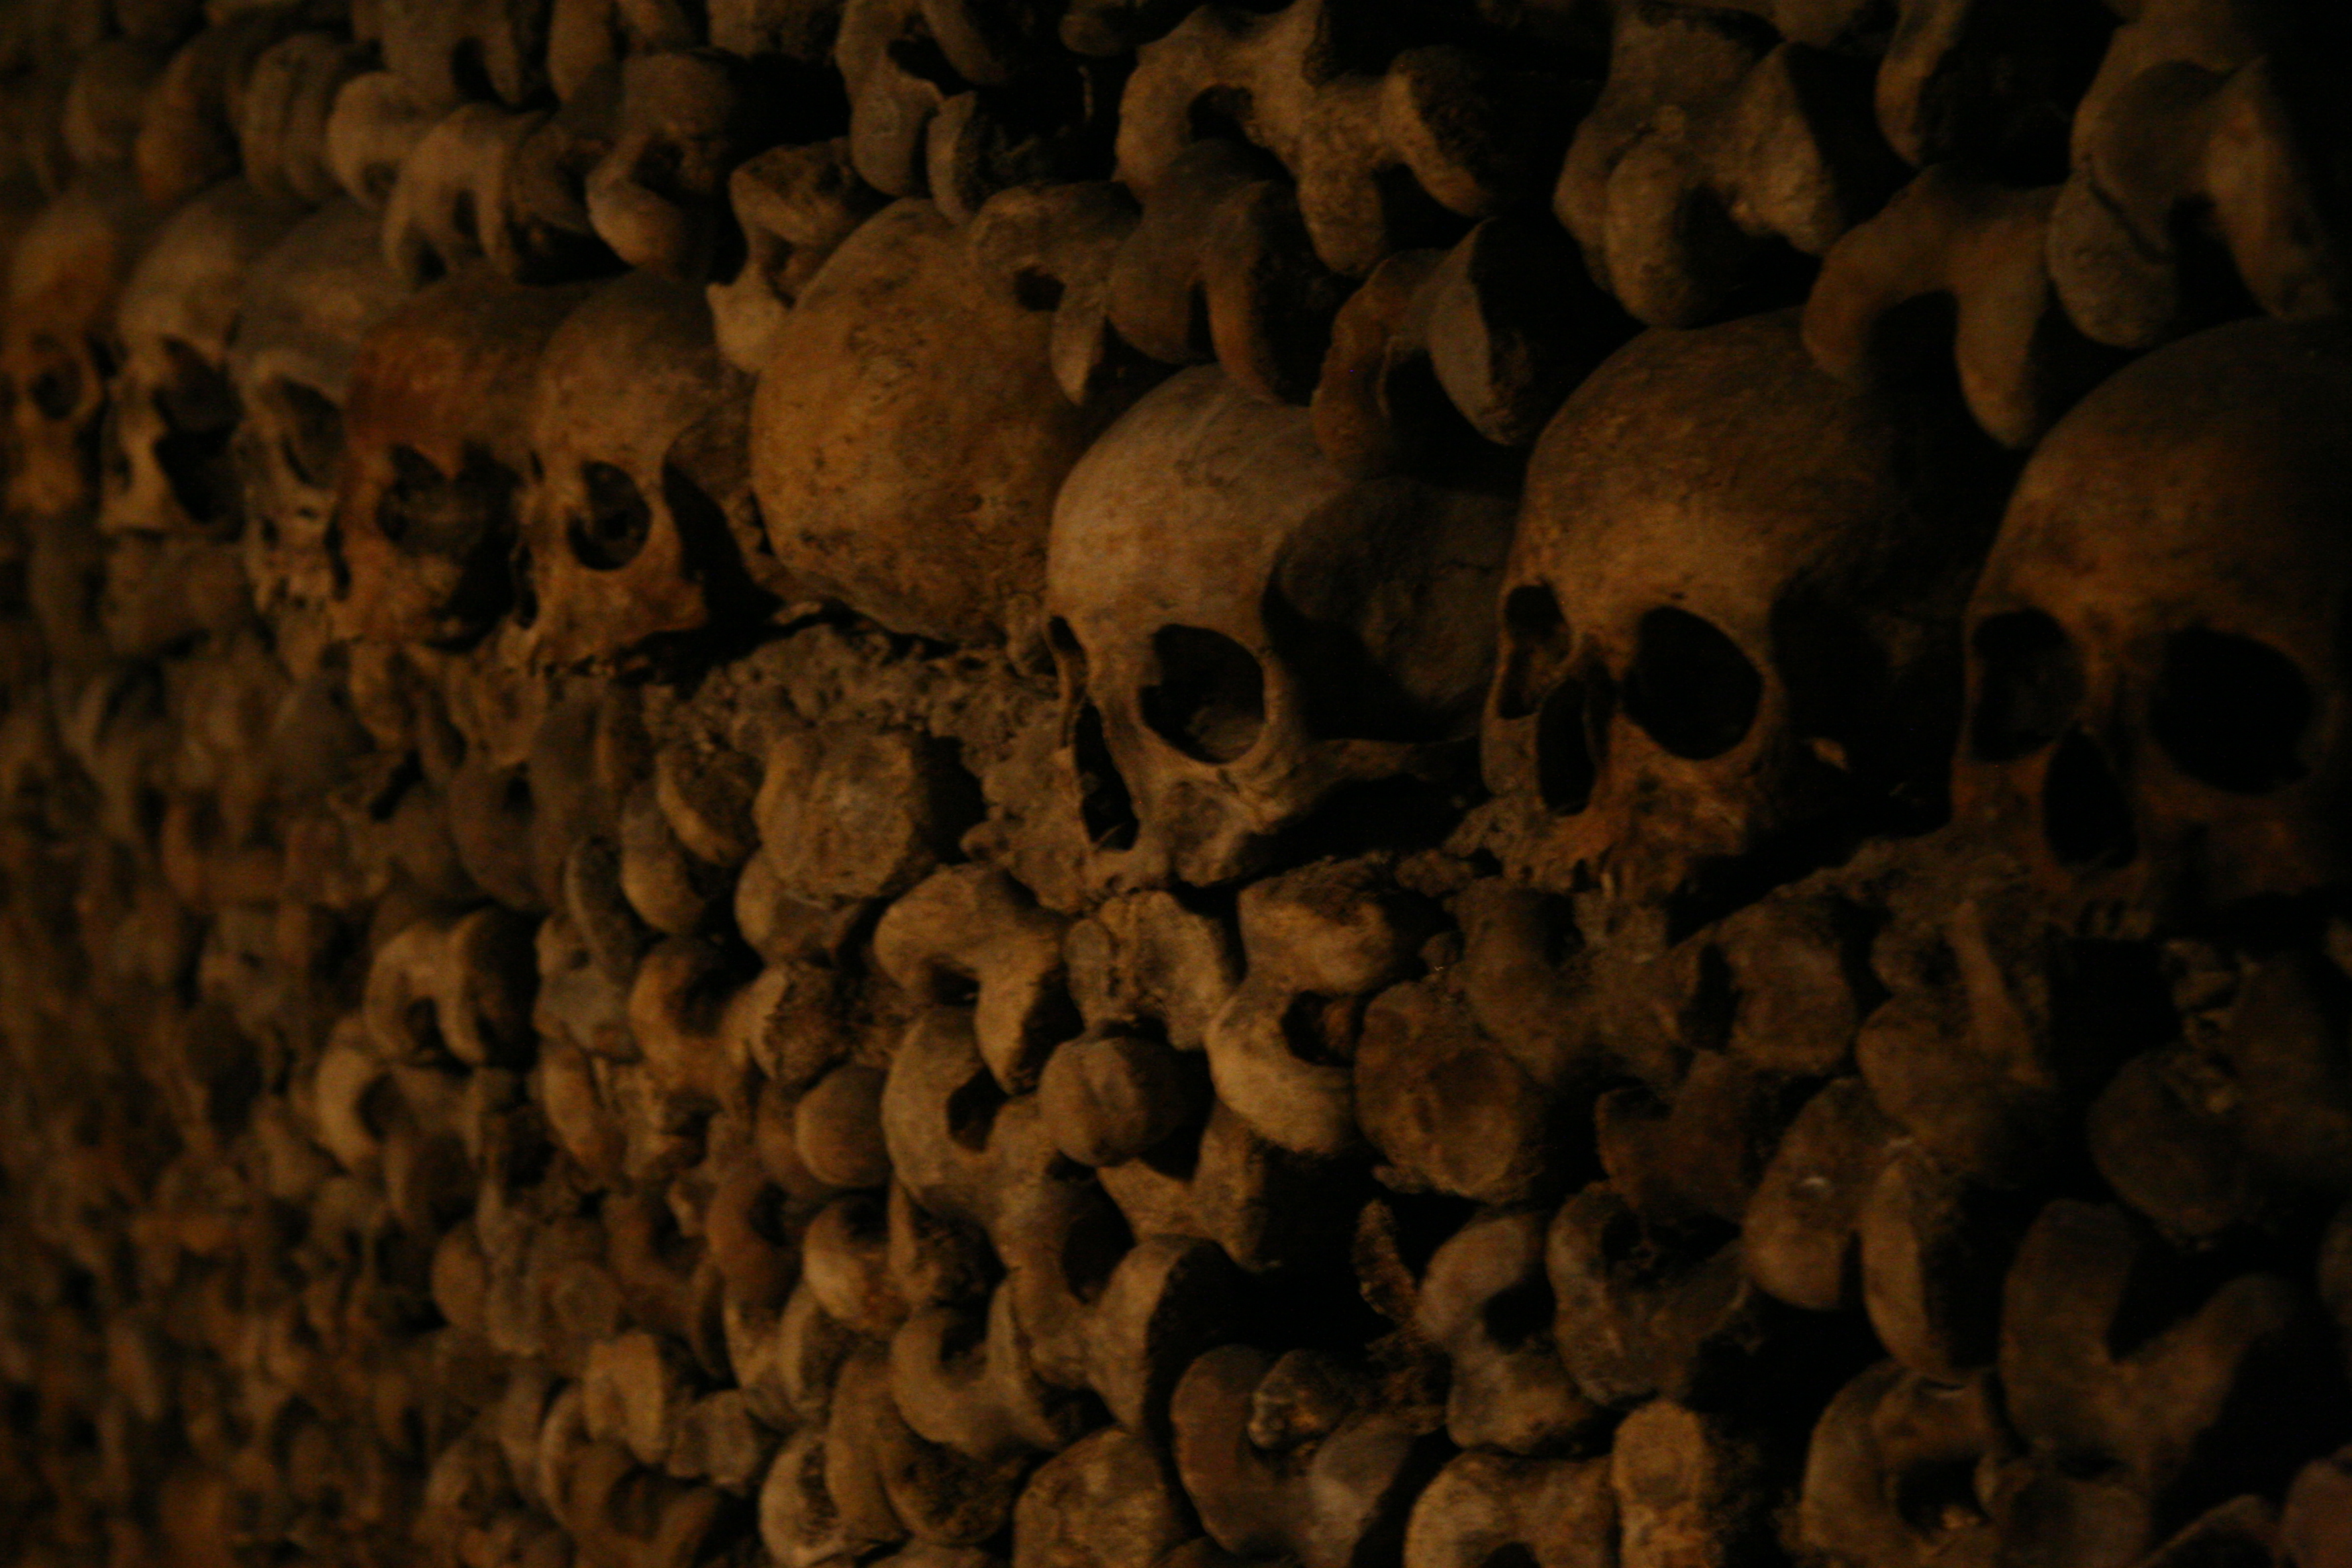
\includegraphics[scale=0.08]{./Ressources/catacombes-Doc_Searls.jpg}
\caption{Le tunnel sous le temple de la guérison // Doc Searls }
\end{center}
\end{figure}

Il s'agit sans aucun doute des anciennes catacombes de la ville. Des hurlements d'hommes résonnent dans le couloir. Enfin, il s'agit, une fois qu'ils ont avancé, de plusieurs couloirs. L'écho rend difficile la localisation des cris, mais après avoir déambulé un peu, ils en trouvent la source.

\subsubsection{La statuette}
Les cris émanent d'une salle

%----------------------------------------------------------------------------

\newpage
\section{Participation au projet}
\subsection{Comment?}
\hypertarget{participation}{}
Creare Mundum vous a plu? 
Envie de partager vos scénarios, vos suggestions ou vos idées?
\newline
Contactez-nous sur la mailing list: \href {mailto:crearemundum@lists.tuxfamily.org}{crearemundum@lists.tuxfamily.org}
\newline
Ou rendez vous sur notre site: \href {http://creare-mundum.tuxfamily.org/} {http://creare-mundum.tuxfamily.org/}
\subsection{Les créateurs}
Voici la liste de ceux qui ont participé au projet Creare Mundum. Leur aide fut, est et sera toujours très précieuse au projet. Merci encore!  
\begin{itemize}
\item Alexandre ’Nobrakal’ Moine 
\item Philippe ’Tymophil’ Aubé 
\item Eliott ’Sulf’ Filippi
\item Émiland ’Derec’ Garrabé
\item Luc H.
\end{itemize}
\subsection{Licence}
Creare Mundum est un projet libre de droit, publié sous la licence Creative Commons BY-SA. C'est à dire que quiconque a la possibilité d'utiliser ce document (ainsi que toute les autres parties du projet), de le redistribuer et de le modifier. La seule obligation est de redistribuer le contenu (modifié ou non) sous les mêmes conditions.
\end{document}